\subsection{Metody uwierzytelniania użytkowników w systemach komputerowych - sposoby, wady, zalety}

\subsubsection{Autentykacja vs. Autoryzacja}

W systemach komputerowych wykorzystywane są dwa podstawowe elementy identyfikacji użytkowników, które ze względu na podobieństwo nazw, są często mylone:

\begin{itemize}
	\item \textbf{Autentykacja} (ang. \textit{authentication}) - Często nazywana uwierzytelnieniem, określa, czy użytkownik jest tym, za kogo faktycznie się podaje, przy wykorzystaniu odpowiedniego rodzaju
	poświadczeń tożsamości.

	\item \textbf{Autoryzacja} (ang. \textit{authorization}) - Definiuje do jakich zasobów bądź operacji użytkownik o
	danej tożsamości ma dostęp.
\end{itemize}

\subsubsection{Klasyfikacja}

Pytanie odnosi się bezpośrednio do pojęcia autentykacji, warto więc pamiętać, że w jego zakres nie wchodzą zagadnienia dotyczące drugiej z metod. Ze względu na wykorzystywane do autentykacji informacje, można podzielić sposoby identyfikacji użytkownika na trzy główne grupy:


\begin{itemize}
	\item \textbf{Coś co wiesz} - Informacje których świadomy jest użytkownik systemu, przykładowo:
	\begin{itemize}
		\item Login i hasło,
		\item Unikatowy klucz dostępu do systemu,
		\item Dane tożsamościowe, np. PESEL, numer dowodu osobistego
	\end{itemize}
	\item \textbf{Coś co masz} - Informacje dostarczane przez urządzenia, które użytkownik posiada, przykładowo:
	\begin{itemize}
		\item Kod weryfikacyjny z SMS lub autentykatora TOTP (Google Authenticator, Authy, itp.). Kody takie są zazwyczaj jednorazowe, oraz posiadają krótki okres ważności (w przypadku TOTP, jest to 30s),
		\item Klucz fizyczny, często podłączany do portów USB (YubiKey) lub w formie karty wkładanej do czytnika (SmartCard), zawierający unikatowy dla użytkownika token umożliwiający autentykację.
	\end{itemize}
	\item \textbf{Coś czym jesteś} - Najnowsza, zyskująca na popularności głównie przez urządzenia mobilne metoda, wykorzystująca dane biometryczne użytkownika, przykładowo:
	\begin{itemize}
		\item Skanery odcisków palca,
		\item Skanery siatkówki,
		\item Rozpoznawanie twarzy.
	\end{itemize}
\end{itemize}

\subsubsection{Połączanie - Wady, zalety}

Metody te stosowane mogą być \textbf{samodzielnie}, lub w \textbf{połączeniu ze sobą}, tworząc rozwiązania autentykacyjne, z których najpopularniejsze to:

\begin{itemize}
	\item \textbf{Login + Hasło} - Najprostszy sposób autentykacji, oparty wyłącznie na wiedzy użytkownika. Jego główną zaletą jest prostota implementacji i wygoda wykorzystania, ponieważ nie wymaga fizycznych poświadczeń tożsamości. Rozwiązanie to jednak nie należy do najbezpieczniejszych, ponieważ przejęcie danych użytkownika umożliwia uzyskanie dostępu do systemu,
	\item \textbf{Weryfikacja dwuetapowa} - Połączenie informacji użytkownika, z informacjami które posiada, najczęściej w formie Login + Hasło + Kod Autentykacyjny. Popularne rozwiązanie stosowane w wielu serwisach internetowych, które po zalogowaniu użytkownika przy pomocy jego informacji, wymaga podania dodatkowego kodu do uzyskania autentykacji w systemie. Rozwiązanie to zapewnia znaczący wzrost bezpieczeństwa w stosunku do klasycznego logowania, kosztem wygody użytkowania, oraz większej trudności implementacji. Największym związanym z nim problemem jest utrata dostępu w momencie utraty urządzenia wykorzystywanego do autentykacji, jednak wiele usług oferuje dodatkowe zabezpieczenie w formie tzw. backup codes - jednorazowych kodów które mogą być wykorzystane w przypadku braku dostępu do urządzenia autentykującego,
	\item \textbf{SmartCard + Hasło} - Metoda wykorzystywana często w systemach firmowych, po wprowadzeniu karty do czytnika użytkownik jest rozpoznawany i proszony o podanie przypisanego do jego konta hasła. Metoda ta zapewnia optymalny poziom bezpieczeństwa, jednak utrata dostępu do karty wymaga utworzenia jej duplikatu, a zazwyczaj również resetu hasła.
\end{itemize}

\begin{figure}[H]
	\centering
	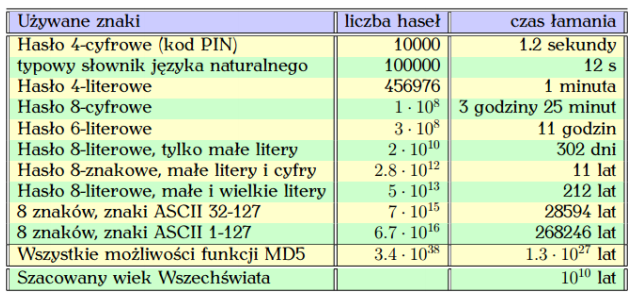
\includegraphics[width=0.8\linewidth]{K1.png}
	\caption{Czas łamania poszczególnych haseł}
\end{figure}